\documentclass[11pt]{article}
\usepackage[a4paper, margin=2.2cm]{geometry}
\usepackage[T1]{fontenc}
\usepackage{helvet}
\renewcommand{\familydefault}{\sfdefault}
\usepackage{parskip}
\usepackage{titlesec}
\usepackage[hidelinks]{hyperref}
\usepackage{tikz}
\usetikzlibrary{arrows.meta, positioning, fit}

\titleformat{\section}{\normalfont\bfseries\large}{}{0pt}{}
\titlespacing{\section}{0pt}{10pt}{5pt}
\titleformat{\subsection}{\normalfont\bfseries}{}{0pt}{}
\titlespacing{\subsection}{0pt}{8pt}{3pt}

\begin{document}

\begin{center}
{\LARGE \bfseries Sinopsis Video: OSI and TCP/IP Models} \\[4pt]
{\large Hafidz Dwi Febrian -- 2406355905}
\end{center}

\vspace{6pt}

\section*{Identitas Video}
\begin{tabular}{ll}
Judul video & : Each layer of the OSI model and TCP/IP explained. \\
Nama channel & : danscourses \\
Link YouTube & : \url{https://youtu.be/kCuyS7ihr_E} \\
Durasi video & : 19:47 \\
Tanggal menonton & : 22 September 2026 \\
\end{tabular}

\section*{Ringkasan Isi Video}

Video ini membahas dua model referensi yang dipakai untuk menjelaskan bagaimana data dikirim dalam sebuah jaringan, yaitu model OSI dan model TCP/IP. OSI punya 7 layer: physical, data link, network, transport, session, presentation, dan application, yang urutannya dari bawah bisa diingat dengan mnemonic ``Please Do Not Throw Sausage Pizza Away''. OSI ini sifatnya lebih ke model konsep untuk memahami cara kerja komunikasi jaringan, bukan sesuatu yang benar-benar diimplementasikan. Yang benar-benar dipakai di internet adalah TCP/IP, yang cuma punya 4 layer: application, transport, internet, dan network access.

\begin{center}
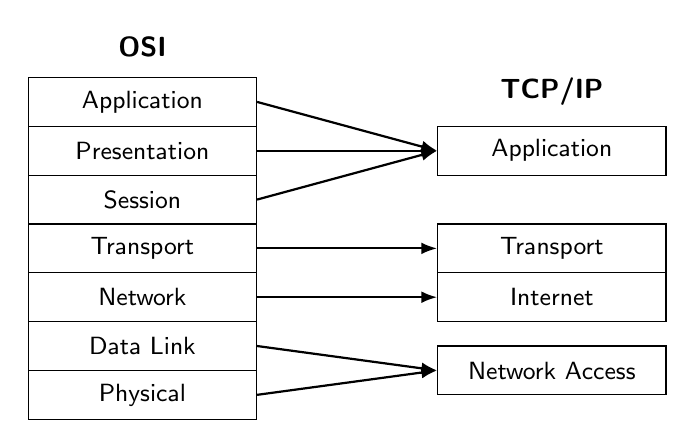
\begin{tikzpicture}[
    box/.style={draw, minimum width=2.9cm, minimum height=0.62cm, align=center, font=\small},
    yscale=1, xscale=1
]
    % OSI stack (7 layers), each row 0.62cm tall, stacked from top y=0 downward
    \node[box] (app)   at (0, 0)      {Application};
    \node[box] (pres)  at (0, -0.62)  {Presentation};
    \node[box] (sess)  at (0, -1.24)  {Session};
    \node[box] (trans) at (0, -1.86)  {Transport};
    \node[box] (net)   at (0, -2.48)  {Network};
    \node[box] (dl)    at (0, -3.10)  {Data Link};
    \node[box] (phy)   at (0, -3.72)  {Physical};

    \node[above=4pt of app, font=\bfseries] {OSI};

    % TCP/IP stack (4 layers), shifted right, same total height, merged rows sized to match
    \node[box] (tapp)  at (5.2, -0.62)  {Application};                         % spans app+pres+sess rows, centered
    \node[box] (ttrans) at (5.2, -1.86) {Transport};                           % same row as OSI transport
    \node[box] (tint)  at (5.2, -2.48)  {Internet};                            % same row as OSI network
    \node[box] (tna)   at (5.2, -3.41)  {Network Access};                      % spans data link + physical rows

    \node[above=4pt of tapp, font=\bfseries] {TCP/IP};

    % grouping arrows from OSI rows into TCP/IP boxes
    \draw[-{Latex[length=2mm]}, thick] (app.east) -- (tapp.west);
    \draw[-{Latex[length=2mm]}, thick] (pres.east) -- (tapp.west);
    \draw[-{Latex[length=2mm]}, thick] (sess.east) -- (tapp.west);
    \draw[-{Latex[length=2mm]}, thick] (trans.east) -- (ttrans.west);
    \draw[-{Latex[length=2mm]}, thick] (net.east) -- (tint.west);
    \draw[-{Latex[length=2mm]}, thick] (dl.east) -- (tna.west);
    \draw[-{Latex[length=2mm]}, thick] (phy.east) -- (tna.west);
\end{tikzpicture}
\end{center}

Seperti terlihat pada gambar, session, presentation, dan application pada OSI digabung jadi satu layer application pada TCP/IP; network menjadi internet; sedangkan data link dan physical digabung menjadi network access.

Hal penting lain dari video ini adalah perubahan bentuk data di tiap layer saat dikirim. Di application layer data masih berupa data biasa. Turun ke transport layer, data dipecah menjadi segment dan ditambahkan informasi port. Turun lagi ke internet layer, data menjadi packet dengan tambahan informasi IP address. Sampai di network access layer, data dibentuk menjadi frame dengan tambahan informasi MAC address, dan akhirnya dikirim sebagai bits melalui media jaringan. Ketika data sampai di perangkat tujuan, proses ini dibalik: bits disusun kembali jadi frame, informasi MAC dilepas, jadi packet, informasi IP dilepas, jadi segment, informasi port dilepas, sampai kembali menjadi data yang bisa dipakai aplikasi penerima. Proses turun ini disebut encapsulation, dan proses naik kembali disebut decapsulation.

\begin{center}
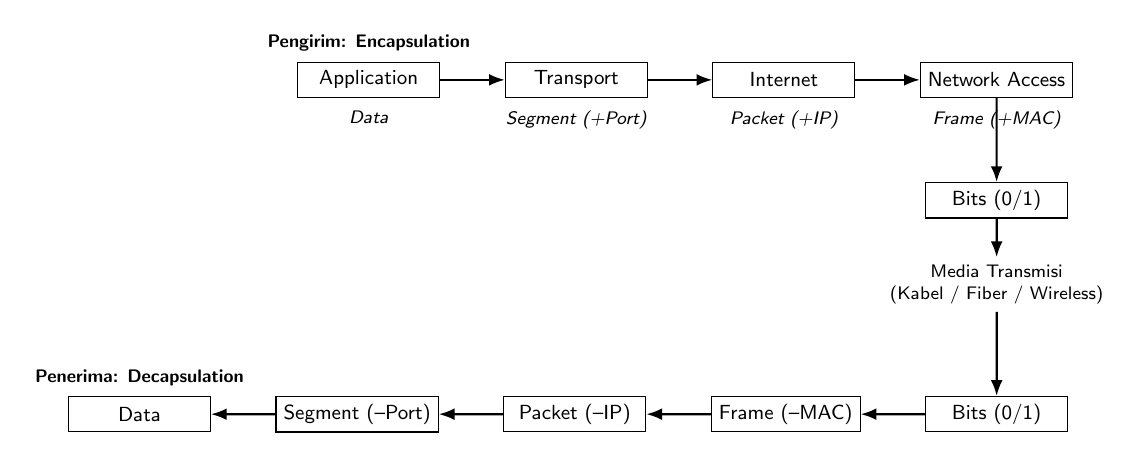
\begin{tikzpicture}[
    scale=0.82, transform shape,
    layerbox/.style={draw, minimum width=2.2cm, minimum height=0.55cm, align=center, font=\small},
    lbl/.style={font=\footnotesize\itshape}
]
    \node[layerbox] (a1) {Application};
    \node[layerbox, right=1.0cm of a1] (t1) {Transport};
    \node[layerbox, right=1.0cm of t1] (i1) {Internet};
    \node[layerbox, right=1.0cm of i1] (n1) {Network Access};

    \node[lbl, below=2pt of a1] {Data};
    \node[lbl, below=2pt of t1] {Segment (+Port)};
    \node[lbl, below=2pt of i1] {Packet (+IP)};
    \node[lbl, below=2pt of n1] {Frame (+MAC)};

    \draw[-{Latex[length=2mm]}, thick] (a1.east) -- (t1.west);
    \draw[-{Latex[length=2mm]}, thick] (t1.east) -- (i1.west);
    \draw[-{Latex[length=2mm]}, thick] (i1.east) -- (n1.west);

    \node[layerbox, below=1.3cm of n1] (bits) {Bits (0/1)};
    \draw[-{Latex[length=2mm]}, thick] (n1.south) -- (bits.north);

    \node[below=0.6cm of bits, font=\footnotesize, align=center] (media) {Media Transmisi\\(Kabel / Fiber / Wireless)};
    \draw[-{Latex[length=2mm]}, thick] (bits.south) -- (media.north);

    \node[layerbox, below=1.3cm of media] (bits2) {Bits (0/1)};
    \draw[-{Latex[length=2mm]}, thick] (media.south) -- (bits2.north);

    \node[layerbox, left=1.0cm of bits2] (n2) {Frame (--MAC)};
    \node[layerbox, left=1.0cm of n2] (i2) {Packet (--IP)};
    \node[layerbox, left=1.0cm of i2] (t2) {Segment (--Port)};
    \node[layerbox, left=1.0cm of t2] (a2) {Data};

    \draw[-{Latex[length=2mm]}, thick] (bits2.west) -- (n2.east);
    \draw[-{Latex[length=2mm]}, thick] (n2.west) -- (i2.east);
    \draw[-{Latex[length=2mm]}, thick] (i2.west) -- (t2.east);
    \draw[-{Latex[length=2mm]}, thick] (t2.west) -- (a2.east);

    \node[above=1pt of a1, font=\footnotesize\bfseries] {Pengirim: Encapsulation};
    \node[above=1pt of a2, font=\footnotesize\bfseries] {Penerima: Decapsulation};
\end{tikzpicture}
\end{center}

\subsection*{Application Layer}
Layer ini berhubungan dengan aplikasi atau layanan yang langsung dipakai user, misalnya HTTP untuk akses website, DNS untuk menerjemahkan nama domain, DHCP untuk mendapatkan IP address otomatis, FTP untuk transfer file, dan SSH untuk koneksi remote. Pada TCP/IP, layer ini sudah mencakup fungsi application, presentation, dan session pada OSI.

\subsection*{Transport Layer}
Layer ini mengatur komunikasi antara aplikasi pengirim dan penerima, lewat dua protokol utama: TCP yang berbasis koneksi dan lebih reliable, serta UDP yang tanpa koneksi dan lebih sederhana. Di layer ini juga ada port number yang menunjukkan aplikasi/layanan yang berkomunikasi, contohnya port 80 untuk HTTP, port 22 untuk SSH, dan port 21 untuk FTP.

\subsection*{Internet Layer}
Berhubungan dengan IP address sebagai alamat logis dan proses routing untuk menentukan jalur data sampai ke tujuan. Di layer ini juga ada konsep QoS (Quality of Service) yang mengatur prioritas traffic, misalnya komunikasi suara butuh pengiriman cepat karena keterlambatan langsung terasa oleh pengguna.

\subsection*{Network Access Layer}
Mencakup fungsi data link dan physical pada OSI yang digabung jadi satu. Bagian data link berhubungan dengan Ethernet, NIC, dan MAC address yang dipakai untuk komunikasi di jaringan lokal serta menjadi bagian informasi pada frame, dan bagian ini juga mengecek frame untuk mendeteksi error saat data diterima. Bagian physical mengirim data dalam bentuk bits melalui media seperti sinyal listrik pada kabel, cahaya pada fiber optic, atau gelombang radio pada koneksi wireless.

\section*{Kesimpulan}

Pengiriman data di jaringan melewati beberapa tahap dan setiap layer punya tugas masing-masing. Yang paling penting untuk dibedakan adalah segment, packet, frame, dan bits karena masing-masing berada di layer yang berbeda: Data $\to$ Segment $\to$ Packet $\to$ Frame $\to$ Bits saat dikirim, lalu dibalik lagi Bits $\to$ Frame $\to$ Packet $\to$ Segment $\to$ Data saat diterima. Selain itu, IP address dan MAC address juga punya fungsi berbeda: IP berhubungan dengan alamat jaringan dan routing, sedangkan MAC dipakai untuk mengirim data ke perangkat di jaringan lokal. TCP dan UDP juga berbeda dari segi cara menangani komunikasi dan reliability-nya.

\section*{Pembelajaran yang Diperoleh}

Dari materi ini saya jadi lebih terbayang hubungan antara masing-masing layer. Sebelumnya istilah seperti IP address, MAC address, TCP, UDP, packet, dan frame terlihat seperti istilah yang berdiri sendiri-sendiri. Setelah melihat pembagiannya berdasarkan layer, jadi lebih gampang untuk mengingatnya karena setiap layer punya tugas masing-masing dan saling melengkapi. Data juga tidak langsung dikirim begitu saja, tapi diberi informasi tambahan di setiap layer sampai akhirnya berubah menjadi bits dan dikirim melalui media jaringan, lalu proses ini dibalik lagi saat sampai di tujuan sampai kembali menjadi data yang bisa dipakai oleh aplikasi. Materi ini berkaitan langsung dengan mata kuliah yang membahas dasar-dasar jaringan komputer, karena pemahaman soal layer ini jadi fondasi sebelum masuk ke topik yang lebih spesifik seperti routing, subnetting, atau keamanan jaringan.

\end{document}
